\documentclass{beamer}

\newcommand{\nfour}{${\cal N}=4\;$}
\newcommand{\ntwo}{${\mathcal N}=2\;$}
\newcommand{\none}{${\mathcal N}=1\,$}
\newcommand{\ntt}{${\mathcal N}=(2,2)\,$}
\newcommand{\nzt}{${\mathcal N}=(0,2)\,$}
\newcommand{\cpn}{CP$^{(N-1)}\,$}
\newcommand{\ca}{{\mathcal A}}
\newcommand{\cell}{{\mathcal L}}
\newcommand{\cw}{{\mathcal W}}
\newcommand{\cs}{{\mathcal S}}
\newcommand{\vp}{\varphi}
\newcommand{\pt}{\partial}
\newcommand{\ve}{\varepsilon}
\newcommand{\gs}{g^{2}}
\newcommand{\zn}{$Z_N$}
\newcommand{\cd}{${\mathcal D}$}
\newcommand{\cde}{{\mathcal D}}
\newcommand{\cf}{${\mathcal F}$}
\newcommand{\cfe}{{\mathcal F}}

\newcommand{\gsim}{\lower.7ex\hbox{$
\;\stackrel{\textstyle>}{\sim}\;$}}
\newcommand{\lsim}{\lower.7ex\hbox{$
\;\stackrel{\textstyle<}{\sim}\;$}}

\renewcommand{\theequation}{\thesection.\arabic{equation}}

%%%%%%%%%%%%%
%%%%%%%%%%%
%% common definitions
\def\stackunder#1#2{\mathrel{\mathop{#2}\limits_{#1}}}
\def\beqn{\begin{eqnarray}}
\def\eeqn{\end{eqnarray}}
\def\nn{\nonumber}
\def\baselinestretch{1.1}
\def\beq{\begin{equation}}
\def\eeq{\end{equation}}
\def\ba{\beq\new\begin{array}{c}}
\def\ea{\end{array}\eeq}
\def\be{\ba}
\def\ee{\ea}
\def\stackreb#1#2{\mathrel{\mathop{#2}\limits_{#1}}}
\def\Tr{{\rm Tr}}
%\newcommand{\gsim}{\lower.7ex\hbox{$\;\stackrel{\textstyle>}{\sim}\;$}}
% \newcommand{\lsim}{\lower.7ex\hbox{$
%\;\stackrel{\textstyle<}{\sim}\;$}}
%\newcommand{\nfour}{${\mathcal N}=4$ }
%\newcommand{\ntwo}{${\mathcal N}=2$ }
\newcommand{\ntwon}{${\mathcal N}=2$}
\newcommand{\ntwot}{${\mathcal N}= \left(2,2\right) $ }
\newcommand{\ntwoo}{${\mathcal N}= \left(0,2\right) $ }
%\newcommand{\none}{${\mathcal N}=1$ }
\newcommand{\nonen}{${\mathcal N}=1$}
%\newcommand{\vp}{\varphi}
%\newcommand{\pt}{\partial}
%\newcommand{\ve}{\varepsilon}
%\newcommand{\gs}{g^{2}}
%\newcommand{\qt}{\tilde q}
\renewcommand{\theequation}{\thesection.\arabic{equation}}

%%
\newcommand{\p}{\partial}
\newcommand{\wt}{\widetilde}
\newcommand{\ov}{\overline}
\newcommand{\mc}[1]{\mathcal{#1}}
\newcommand{\md}{\mathcal{D}}

\newcommand{\GeV}{{\rm GeV}}
\newcommand{\eV}{{\rm eV}}
\newcommand{\Heff}{{\mathcal{H}_{\rm eff}}}
\newcommand{\Leff}{{\mathcal{L}_{\rm eff}}}
\newcommand{\el}{{\rm EM}}
\newcommand{\uflavor}{\mathbf{1}_{\rm flavor}}
\newcommand{\lgr}{\left\lgroup}
\newcommand{\rgr}{\right\rgroup}

\newcommand{\Mpl}{M_{\rm Pl}}
\newcommand{\suc}{{{\rm SU}_{\rm C}(3)}}
\newcommand{\sul}{{{\rm SU}_{\rm L}(2)}}
\newcommand{\sutw}{{\rm SU}(2)}
\newcommand{\suth}{{\rm SU}(3)}
\newcommand{\ue}{{\rm U}(1)}
%%%%%%%%%%%%%%%%%%%%%%%%%%%%%%%%%%%%%%%
%  Slash character...
\def\slashed#1{\setbox0=\hbox{$#1$}             % set a box for #1
   \dimen0=\wd0                                 % and get its size
   \setbox1=\hbox{/} \dimen1=\wd1               % get size of /
   \ifdim\dimen0>\dimen1                        % #1 is bigger
      \rlap{\hbox to \dimen0{\hfil/\hfil}}      % so center / in box
      #1                                        % and print #1
   \else                                        % / is bigger
      \rlap{\hbox to \dimen1{\hfil$#1$\hfil}}   % so center #1
      /                                         % and print /
   \fi}                                        %

%%EXAMPLE:  $\slashed{E}$ or $\slashed{E}_{t}$

%%

\newcommand{\LN}{\Lambda_\text{SU($N$)}}
\newcommand{\sunu}{{\rm SU($N$) $\times$ U(1) }}
\newcommand{\sunun}{{\rm SU($N$) $\times$ U(1)}}
\def\cfl {$\text{SU($N$)}_{\rm C+F}$ }
\def\cfln {$\text{SU($N$)}_{\rm C+F}$}
\newcommand{\mUp}{m_{\rm U(1)}^{+}}
\newcommand{\mUm}{m_{\rm U(1)}^{-}}
\newcommand{\mNp}{m_\text{SU($N$)}^{+}}
\newcommand{\mNm}{m_\text{SU($N$)}^{-}}
\newcommand{\AU}{\mc{A}^{\rm U(1)}}
\newcommand{\AN}{\mc{A}^\text{SU($N$)}}
\newcommand{\aU}{a^{\rm U(1)}}
\newcommand{\aN}{a^\text{SU($N$)}}
\newcommand{\baU}{\ov{a}{}^{\rm U(1)}}
\newcommand{\baN}{\ov{a}{}^\text{SU($N$)}}
\newcommand{\lU}{\lambda^{\rm U(1)}}
\newcommand{\lN}{\lambda^\text{SU($N$)}}
%\newcommand{\Tr}{{\rm Tr\,}}
\newcommand{\bxir}{\ov{\xi}{}_R}
\newcommand{\bxil}{\ov{\xi}{}_L}
\newcommand{\xir}{\xi_R}
\newcommand{\xil}{\xi_L}
\newcommand{\bzl}{\ov{\zeta}{}_L}
\newcommand{\bzr}{\ov{\zeta}{}_R}
\newcommand{\zr}{\zeta_R}
\newcommand{\zl}{\zeta_L}
\newcommand{\nbar}{\ov{n}}

\newcommand{\CPC}{CP$^{N-1}$)$\times$C }
\newcommand{\CPCn}{CP$^{N-1}$)$\times$C}

\newcommand{\lar}{\lambda_R}
\newcommand{\lal}{\lambda_L}
\newcommand{\larl}{\lambda_{R,L}}
\newcommand{\lalr}{\lambda_{L,R}}
\newcommand{\bla}{\ov{\lambda}}
\newcommand{\blar}{\ov{\lambda}{}_R}
\newcommand{\blal}{\ov{\lambda}{}_L}
\newcommand{\blarl}{\ov{\lambda}{}_{R,L}}
\newcommand{\blalr}{\ov{\lambda}{}_{L,R}}

\newcommand{\bgamma}{\ov{\gamma}}
\newcommand{\bpsi}{\ov{\psi}{}}
\newcommand{\bphi}{\ov{\phi}{}}
\newcommand{\bxi}{\ov{\xi}{}}

\newcommand{\ff}{\mc{F}}
\newcommand{\bff}{\ov{\mc{F}}}

\newcommand{\eer}{\epsilon_R}
\newcommand{\eel}{\epsilon_L}
\newcommand{\eerl}{\epsilon_{R,L}}
\newcommand{\eelr}{\epsilon_{L,R}}
\newcommand{\beer}{\ov{\epsilon}{}_R}
\newcommand{\beel}{\ov{\epsilon}{}_L}
\newcommand{\beerl}{\ov{\epsilon}{}_{R,L}}
\newcommand{\beelr}{\ov{\epsilon}{}_{L,R}}

\newcommand{\bi}{{\bar \imath}}
\newcommand{\bj}{{\bar \jmath}}
\newcommand{\bk}{{\bar k}}
\newcommand{\bl}{{\bar l}}
\newcommand{\bmm}{{\bar m}}
\newcommand{\bp}{{\bar p}}
\newcommand{\bkk}{{\bar k}}
\newcommand{\br}{{\bar r}}

\newcommand{\nz}{{n^{(0)}}}
\newcommand{\no}{{n^{(1)}}}
\newcommand{\bnz}{{\ov{n}{}^{(0)}}}
\newcommand{\bno}{{\ov{n}{}^{(1)}}}
\newcommand{\Dz}{{D^{(0)}}}
\newcommand{\Do}{{D^{(1)}}}
\newcommand{\bDz}{{\ov{D}{}^{(0)}}}
\newcommand{\bDo}{{\ov{D}{}^{(1)}}}
\newcommand{\sigz}{{\sigma^{(0)}}}
\newcommand{\sigo}{{\sigma^{(1)}}}
\newcommand{\bsigz}{{\ov{\sigma}{}^{(0)}}}
\newcommand{\bsigo}{{\ov{\sigma}{}^{(1)}}}

\newcommand{\rrenz}{{r_\text{ren}^{(0)}}}
\newcommand{\bren}{{\beta_\text{ren}}}

\newcommand{\mbps}{m_{\text{\tiny BPS}}}
\newcommand{\W}{\mathcal{W}}
\newcommand{\M}{\mathcal{M}}
\newcommand{\bM}{\ov{\mathcal{M}}{}}
\newcommand{\Q}{\mathcal{Q}}
\newcommand{\bQ}{\ov{\mathcal{Q}}{}}
\newcommand{\D}{\mathcal{D}}
\newcommand{\hsigma}{{\hat{\sigma}}}
\newcommand{\V}{\mathcal{V}}


\usefonttheme{serif}
\usetheme{AnnArbor}

\setbeamertemplate{background canvas}[vertical shading][bottom=green!30,top=yellow!30]
\setbeamertemplate{blocks}[rounded][shadow=true]

\setbeamercolor{normal text}{fg=blue!80}
\setbeamercolor{alerted text}{fg=orange!90}
\setbeamercolor{math text}{fg=red!90}

\title[Two-dim. --- four-dim. duality]
      {Two-dimensional --- four-dimensional duality:\\
	Towers of kinks $\leftrightarrow$ towers of monopoles\\ 
		in $\mathcal{N}=2$ theories}

\author{Pavel A. Bolokhov}

\date{May 8, 2012}

\institute[UMN \& SPbSU]{University of Minnesota ~~$\cdot$~~ St.Petersburg State University}

\begin{document}

\maketitle

%%%%%%%%%%%%%%%%%%%%%%%%%%%%%%%%%%%%%%%%%%%%%%%%%%%%%%%%%%%%%%%%%%
%%%%%%%%%%%%%%%%%%%%%%%%%%%%%%%%%%%%%%%%%%%%%%%%%%%%%%%%%%%%%%%%%%
\section{Introduction}
%%%%%%%%%%%%%%%%%%%%%%%%%%%%%%%%%%%%%%%%%%%%%%%%%%%%%%%%%%%%%%%%%%
%%%%%%%%%%%%%%%%%%%%%%%%%%%%%%%%%%%%%%%%%%%%%%%%%%%%%%%%%%%%%%%%%%


%%%%%%%%%%%%%%%%%%%%%%%%%%%%%%%%%%%%%%%%%%%%%%%%%%%%%%%%%%%%%%%%%%
\begin{frame}{}


	Two-dimensional models have interesting similarities to 4-d gauge theories
\vspace{0.4cm}

	CP$^{N-1}$ theory has been shown to have chiral symmetry breaking, mass gap,
	asymptotic freedom, {\it etc} and all these properties are much easier to show
	in two dimensions 
\vspace{0.4cm}

	In general, two-dimensional theories are simpler and two-dimensional methods
	are more powerful

\end{frame}


%%%%%%%%%%%%%%%%%%%%%%%%%%%%%%%%%%%%%%%%%%%%%%%%%%%%%%%%%%%%%%%%%%
\begin{frame}{}

	There is also a two-dimensional --- four-dimensional duality of their BPS spectra

\vspace{7mm}
\begin{columns}[t]
	\column{5cm}
	$ \mathcal{N}=2 $\,  $ N_c = N_f $ SYM 
	in four dimensions at the root
	of the first baryonic Higgs branch

	\column{0.5cm}
	\vspace{2mm}
	$ \longleftrightarrow $

	\column{5cm}
	$ \mathcal{N}=(2,2) $ CP$^{N-1}$ theory
	in two dimensions
\end{columns}

\vspace{5mm}
\begin{columns}[t]
	\column{5.0cm}
		\centering
		$ \downarrow $

	\column{0.5cm}

	\column{5.0cm}
		\centering
		$ \downarrow $
\end{columns}

\vspace{5mm}
\begin{columns}[t]
	\column{5cm}
	supports non-Abelian
	vortex strings

	\column{0.5cm}

	\column{5cm}
	kinks interpolate
	between worldsheet vacua
\end{columns}

\vspace{7mm}
\begin{columns}[t]
	\column{5cm}
	\centering
	monopoles\\[7mm]
	strings

	\column{0.5cm}
	$ \longleftrightarrow $\\[7mm]
	$ \longleftrightarrow $
	
	\column{5cm}
	\centering
	kinks\\[7mm]
	vacua
\end{columns}


\end{frame}


%%%%%%%%%%%%%%%%%%%%%%%%%%%%%%%%%%%%%%%%%%%%%%%%%%%%%%%%%%%%%%%%%%
%%%%%%%%%%%%%%%%%%%%%%%%%%%%%%%%%%%%%%%%%%%%%%%%%%%%%%%%%%%%%%%%%%
\section{Two-dimensional analysis}
%%%%%%%%%%%%%%%%%%%%%%%%%%%%%%%%%%%%%%%%%%%%%%%%%%%%%%%%%%%%%%%%%%
%%%%%%%%%%%%%%%%%%%%%%%%%%%%%%%%%%%%%%%%%%%%%%%%%%%%%%%%%%%%%%%%%%


%%%%%%%%%%%%%%%%%%%%%%%%%%%%%%%%%%%%%%%%%%%%%%%%%%%%%%%%%%%%%%%%%%
\begin{frame}{}

	At weak coupling the Seiberg-Witten theory contains
	\alert{Quarks}, \alert{W-bosons}, \alert{Monopoles}, \alert{Dyons} and \alert{bound states}

\vspace{7mm}
	At strong coupling --- we consider CP$^{N-1}$ theory\\
	Strong coupling spectrum is accessible via the mirror theory
\end{frame}


%%%%%%%%%%%%%%%%%%%%%%%%%%%%%%%%%%%%%%%%%%%%%%%%%%%%%%%%%%%%%%%%%%
\begin{frame}[t]{}

\vspace{2mm}
	\underline{CP$^{N-1}$ theory with {\it twisted} masses:}

\begin{align*}
%
	&
	r \lgr \big| \mc{D}_\mu \, n^l \big|^2  ~+~ | \sigma \,-\, m^l |^2 \, \big| n^l \big|^2 
		~+~ i\, D\, \big( \big| n^l \big|^2 \,-\, 1 \big) ~+~ ... \rgr
	\\
%
	&
	~+~ \frac{1}{4e^2}\, F_{\mu\nu}^2 ~+~ \frac{1}{e^2}\, \big|\p_\mu \sigma\big|^2 
	~+~ \frac{1}{2e^2}\, D^2 ~+~ ...\,,
\end{align*}

	in the $ e^2 ~\to~ \infty $ limit

\vspace{7mm}
\only<1>{
	The theory has $ N $ vacua --- both classically and exactly
}
\only<2->{
	CP$^{N-1}$ model with $ \mc{Z}_N $ twisted masses
\[
	m_l  ~~=~~ m_0 \cdot e^{2\pi i l / N}
\]
	in this case $ \mc{Z}_N ~\subset~ U_R(1) $ remains unbroken

}
\end{frame}


%%%%%%%%%%%%%%%%%%%%%%%%%%%%%%%%%%%%%%%%%%%%%%%%%%%%%%%%%%%%%%%%%%
\begin{frame}{Exact superpotential}

	The theory possesses an ``exact'' superpotential of
	Veneziano-Yankielowicz type
\[
	\W_\text{eff} ~~=~~ -\,i\,\tau\hsigma
			~~+~~ \frac{1}{2\pi}\, \sum_l\, \big( \,\hsigma \,-\, m_l\, \big)
				\lgr \ln\, \frac{\hsigma \,-\, m_l}{\mu} ~-~ 1 \rgr
\]
	\flushright{$\mu$ = UV cut-off scale}

\end{frame}


%%%%%%%%%%%%%%%%%%%%%%%%%%%%%%%%%%%%%%%%%%%%%%%%%%%%%%%%%%%%%%%%%%
\begin{frame}{Exact superpotential}

	Vacuum values:
\[
	\W_\text{eff} ~~=~~ -\, \frac{1}{2\pi}\, \lgr N \,\sigma_p  ~+~  \sum_l\, m_l\; \ln\; ( \sigma_p \,-\, m_l ) \rgr
\]

	where
\begin{columns}
\column{.5\textwidth}
\[
	\sigma_p ~~=~~ \sigma_0 \cdot e^{2 \pi i p / N}
\]
\[
	\sigma_0 ~~=~~ \sqrt[N]{ 1 \,+\, m_0^N }
\]

\column{.5\textwidth}
\vspace{2mm}
\begin{block}{vacuum equation}
\[
	\prod_l\, (\, \sigma \,-\, m_l \,) ~~=~~ 1\,.
\]
\end{block}

\end{columns}

\end{frame}


%%%%%%%%%%%%%%%%%%%%%%%%%%%%%%%%%%%%%%%%%%%%%%%%%%%%%%%%%%%%%%%%%%
\begin{frame}{Mirror dual of CP$^{N-1}$}

	The mirror dual is the affine Toda theory
\[
	\W_\text{mirror}^\text{CP$^{N-1}$} ~~=~~
	-\, \frac{1}{2\pi}
	\lgr  
		x_1 ~+~ x_2 ~+~ ... ~+~ x_n ~+~
		\sum\, m_l\; \ln\, x_l 
	\rgr,
\]
\vspace{-4mm}
\[
	x_1\; x_2\; ...\; x_n ~~=~~ 1
\]
	Only the superpotential is known in that theory

\vspace{7mm}
	The vacuum values coincide with $ \W_\text{eff}(\sigma_p) $ upon
	identification
\[
	x_l^{(p)} ~~=~~ \sigma_p \,-\, m_l
\]

\end{frame}


%%%%%%%%%%%%%%%%%%%%%%%%%%%%%%%%%%%%%%%%%%%%%%%%%%%%%%%%%%%%%%%%%%
\begin{frame}{}

	Based on work of K.Hori and C.Vafa, $ N $ mirror kinks
	can be found at strong coupling

\[
	| \,m_k\, | ~~\leq~~ 1
\]

	Limiting to the sector interpolating between $0^\text{th}$ and $ 1^\text{st} $ vacua

\[
	\mc{Z} ~~=~~ \W(\sigma_1) ~-~ \W(\sigma_0) ~+~ i\,m_k\,,
	\qquad\qquad k \,=\, 0\,, ..., N-1,
\]

\end{frame}


%%%%%%%%%%%%%%%%%%%%%%%%%%%%%%%%%%%%%%%%%%%%%%%%%%%%%%%%%%%%%%%%%%
\begin{frame}{}

\begin{center}
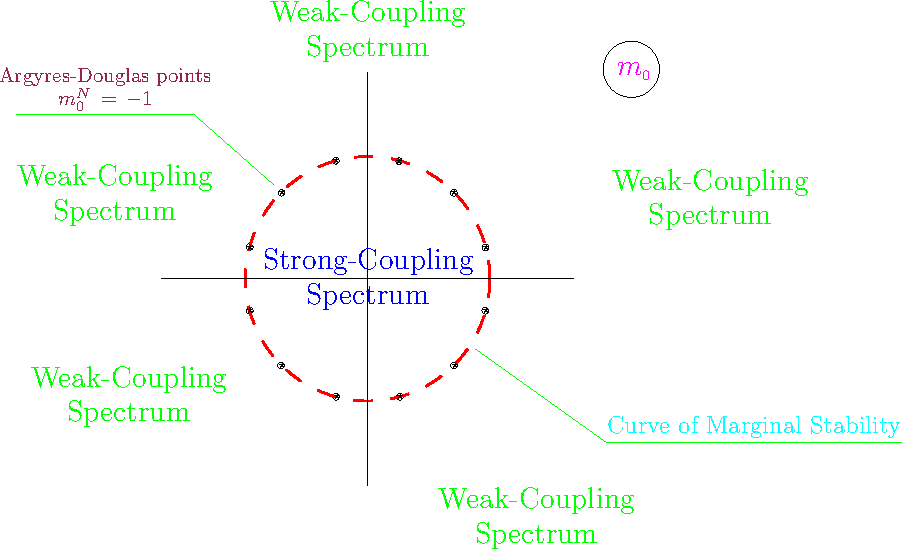
\includegraphics[width=10cm]{mplane.pdf}
\end{center}

\end{frame}


%%%%%%%%%%%%%%%%%%%%%%%%%%%%%%%%%%%%%%%%%%%%%%%%%%%%%%%%%%%%%%%%%%
\begin{frame}{}

	The spectrum

\begin{block}{}
\[
	\mc{Z} ~~=~~ \W(\sigma_1) ~-~ \W(\sigma_0) ~+~ i\,m_k\,,
	\qquad\qquad k \,=\, 0\,, ..., N-1,
\]
\end{block}

	describes $ N $ dyonic kinks 
	(of either CP$^{N-1}$ or the mirror theory)
	in the fundamental of $\text{SU($N$)}$

	\pause
\begin{block}{Question:} 
	\qquad\qquad
	What happens to them at weak coupling?
\end{block}

	\pause
\begin{block}{}
	\qquad\qquad
	What states do they correspond to?
\end{block}

\end{frame}


%%%%%%%%%%%%%%%%%%%%%%%%%%%%%%%%%%%%%%%%%%%%%%%%%%%%%%%%%%%%%%%%%%
\begin{frame}{}

	Previously known picture

\begin{block}{Weak coupling:}  

\vspace{2mm}
	\qquad\qquad
	\qquad\qquad
	$ \Q_{ik} $,\quad $ \M_{ik} $,\quad $ \D_{ik}^n $\\[0.5cm]

	\qquad\qquad
	\qquad\qquad
	$ \D_{ik}^n ~+~ Q $ \quad---\quad bound states
\vspace{1mm}
\end{block}

\begin{block}{}
$
	\Q_{ik}  ~~~=~~  i\, (\, m_i \,-\, m_k \,)
$\\[4mm]

$ \M_{ik} $ \,~---~~ purely topological kink interpolating from $(k) ~~\rightarrow~~ (i)$
\\[4mm]

$
	\D_{ik}^n  ~~~=~~ \M_{ik}  ~~+~~ i\, n\, (\, m_i \,-\, m_k \,)
$ 
	~~---~~ tower of dyonic kinks upon\\
\hspace{7cm} quasiclassical quantization
\vspace{1mm}
\end{block}

\end{frame}


%%%%%%%%%%%%%%%%%%%%%%%%%%%%%%%%%%%%%%%%%%%%%%%%%%%%%%%%%%%%%%%%%%
\begin{frame}{$\text{CP}^2$ theory}

	We focus on $\text{CP}^2$ model --- the first non-trivial theory.\\[2mm]

	We find the curves of marginal stability ({\it c.m.s.}) --- analogues of wall crossing --- 
	for this model, where the spectrum can change due to decays

	\pause
\begin{block}{}
\vspace{2mm}

	\alert{\it c.m.s.} are a supersymmetric version of a ``phase transition''\\[1mm]
	there are practically no phase transitions in supersymmetric theories
	except for, perhaps, when supersymmetry is broken, 
	or for theories with $ N_c ~\to~ \infty $
	
\vspace{2mm}
\end{block}

\end{frame}


%%%%%%%%%%%%%%%%%%%%%%%%%%%%%%%%%%%%%%%%%%%%%%%%%%%%%%%%%%%%%%%%%%
\begin{frame}{Moduli space of $\text{CP}^2$ --- plane of $ m_0 $}

\vspace{-1.0cm}
\begin{center}
\hspace{-9mm}
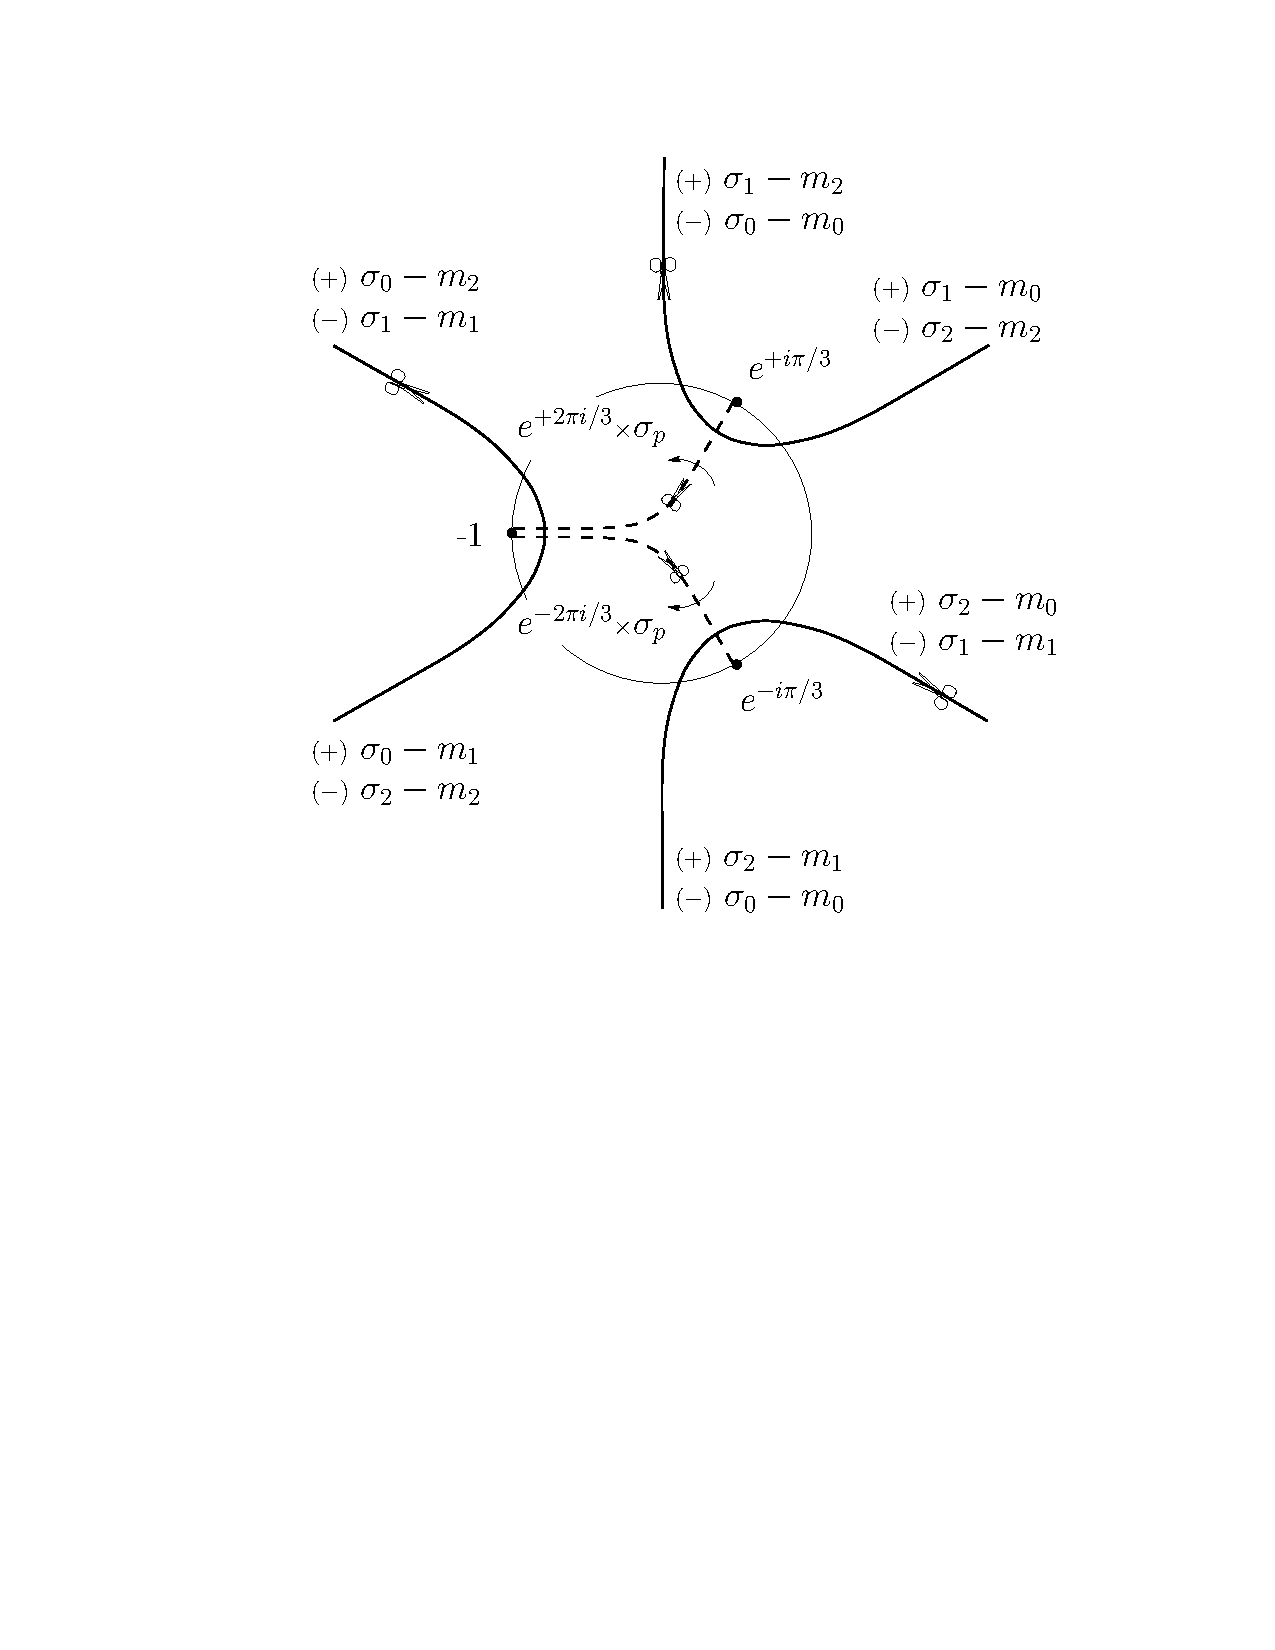
\includegraphics[width=10cm]{fcp2.pdf}
\end{center}

\vspace{-6cm}
\centering
	there are three $ \mc{Z}_3 $--equivalent sectors

\end{frame}


%%%%%%%%%%%%%%%%%%%%%%%%%%%%%%%%%%%%%%%%%%%%%%%%%%%%%%%%%%%%%%%%%%
\begin{frame}{}

	So we choose only one topological sector:\\[3mm]

\begin{block}
\qquad\qquad\qquad\qquad
	kinks: \qquad\qquad $ (0) ~~~\longrightarrow~~~ (1) $
\vspace{2mm}
\end{block}

\vspace{2mm}
	and one sector in $ m_0 $-plane:
\vspace{2mm}

\begin{block}{}
\begin{columns}[c]
\column{6cm}
\centering
	\vspace{-2mm}
	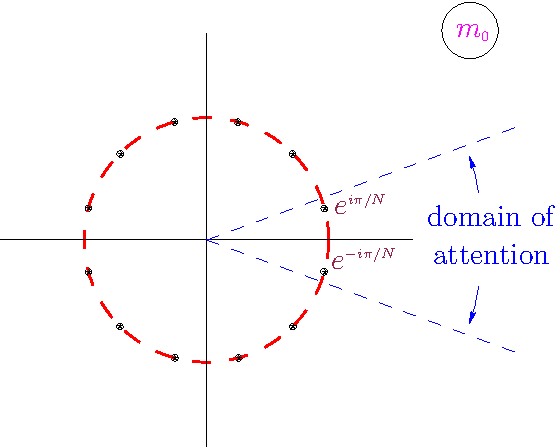
\includegraphics[width=6cm]{domain.pdf}
\column{5cm}
	the other two sectors are completely equivalent\\[4mm]
	other kinks have the same masses, 
	just central charges shifted by a phase
\end{columns}
\vspace{2mm}
\end{block}

\end{frame}


%%%%%%%%%%%%%%%%%%%%%%%%%%%%%%%%%%%%%%%%%%%%%%%%%%%%%%%%%%%%%%%%%%
%%%%%%%%%%%%%%%%%%%%%%%%%%%%%%%%%%%%%%%%%%%%%%%%%%%%%%%%%%%%%%%%%%
\section{Spectrum}
%%%%%%%%%%%%%%%%%%%%%%%%%%%%%%%%%%%%%%%%%%%%%%%%%%%%%%%%%%%%%%%%%%
%%%%%%%%%%%%%%%%%%%%%%%%%%%%%%%%%%%%%%%%%%%%%%%%%%%%%%%%%%%%%%%%%%


%%%%%%%%%%%%%%%%%%%%%%%%%%%%%%%%%%%%%%%%%%%%%%%%%%%%%%%%%%%%%%%%%%
\begin{frame}{Weak coupling spectrum}

\begin{columns}[c]
\column{5cm}
\centering

\uncover<2->{decays}

	\vspace{17mm}

\uncover<3->{
	decay all\\
	but one
	}

	\vspace{5mm}
\uncover<4->{all decay}

\column{1cm}

	\vspace{-2mm}

\quad
\uncover<2->{$ \Longleftarrow $}

	\vspace{14mm}

\quad
\uncover<3->{$ \Longleftarrow $}

	\vspace{3mm}

\quad
\uncover<4->{$ \Longleftarrow $}

	\vspace{4mm}


\column{5cm}
\centering

	$ \Q_{ik} $

	\vspace{7mm}

	$ \M_{10} $

	\vspace{7mm}

	$ \D_{10}^{(n)} $

	\vspace{7mm}

	$ \D_{10}^{(n)}\,\Q_{02} $

\end{columns}

\end{frame}


%%%%%%%%%%%%%%%%%%%%%%%%%%%%%%%%%%%%%%%%%%%%%%%%%%%%%%%%%%%%%%%%%%
\begin{frame}{Strong coupling spectrum}

\begin{columns}[t]
\column{10cm}
\uncover<5->{
$
	\hspace{0.5mm}
	\M_{10}  
	\hspace{3.5mm}
	\Longleftarrow
$
}
$
	\hspace{5.5mm}
	\W_1  ~~-~~  \W_0  ~~+~~  i\,m_0
$
\uncover<4->{
	\hspace{3.5mm}
	--- 
	\hspace{3mm}
	next lightest
}
	\\[12mm]

\uncover<7->{
$
	\hspace{2mm}
	\D_{10}  
	\hspace{4.8mm}
	\Longleftarrow
$
}
$
	\hspace{5mm}
	\W_1  ~~-~~  \W_0  ~~+~~  i\,m_1
$
\uncover<6->{
	\hspace{2mm}
	--- 
	\hspace{3mm}
	the heavier
}
	\\[12mm]

\uncover<3->{
	decays
$
	\hspace{1.9mm}
	\Leftarrow=
$
}
$
	\hspace{4.6mm}
	\W_1  ~~-~~  \W_0  ~~+~~  i\,m_2
$
\uncover<2->{
	\hspace{3mm}
	---
	\hspace{3mm}
	the lightest
}
	\\[8mm]

\column{2cm}
\centering
\small
\uncover<8->
{
	$ \longleftarrow $\\[-0.8mm]
	build\\
	their own\\
	tower\\[-0.8mm]
	$ \longleftarrow $\\
}

\end{columns}


\end{frame}


%%%%%%%%%%%%%%%%%%%%%%%%%%%%%%%%%%%%%%%%%%%%%%%%%%%%%%%%%%%%%%%%%%
\begin{frame}{\it c.m.s.}

\begin{columns}
\column{2cm}

\column{20cm}
\begin{center}
\vspace{-17cm}
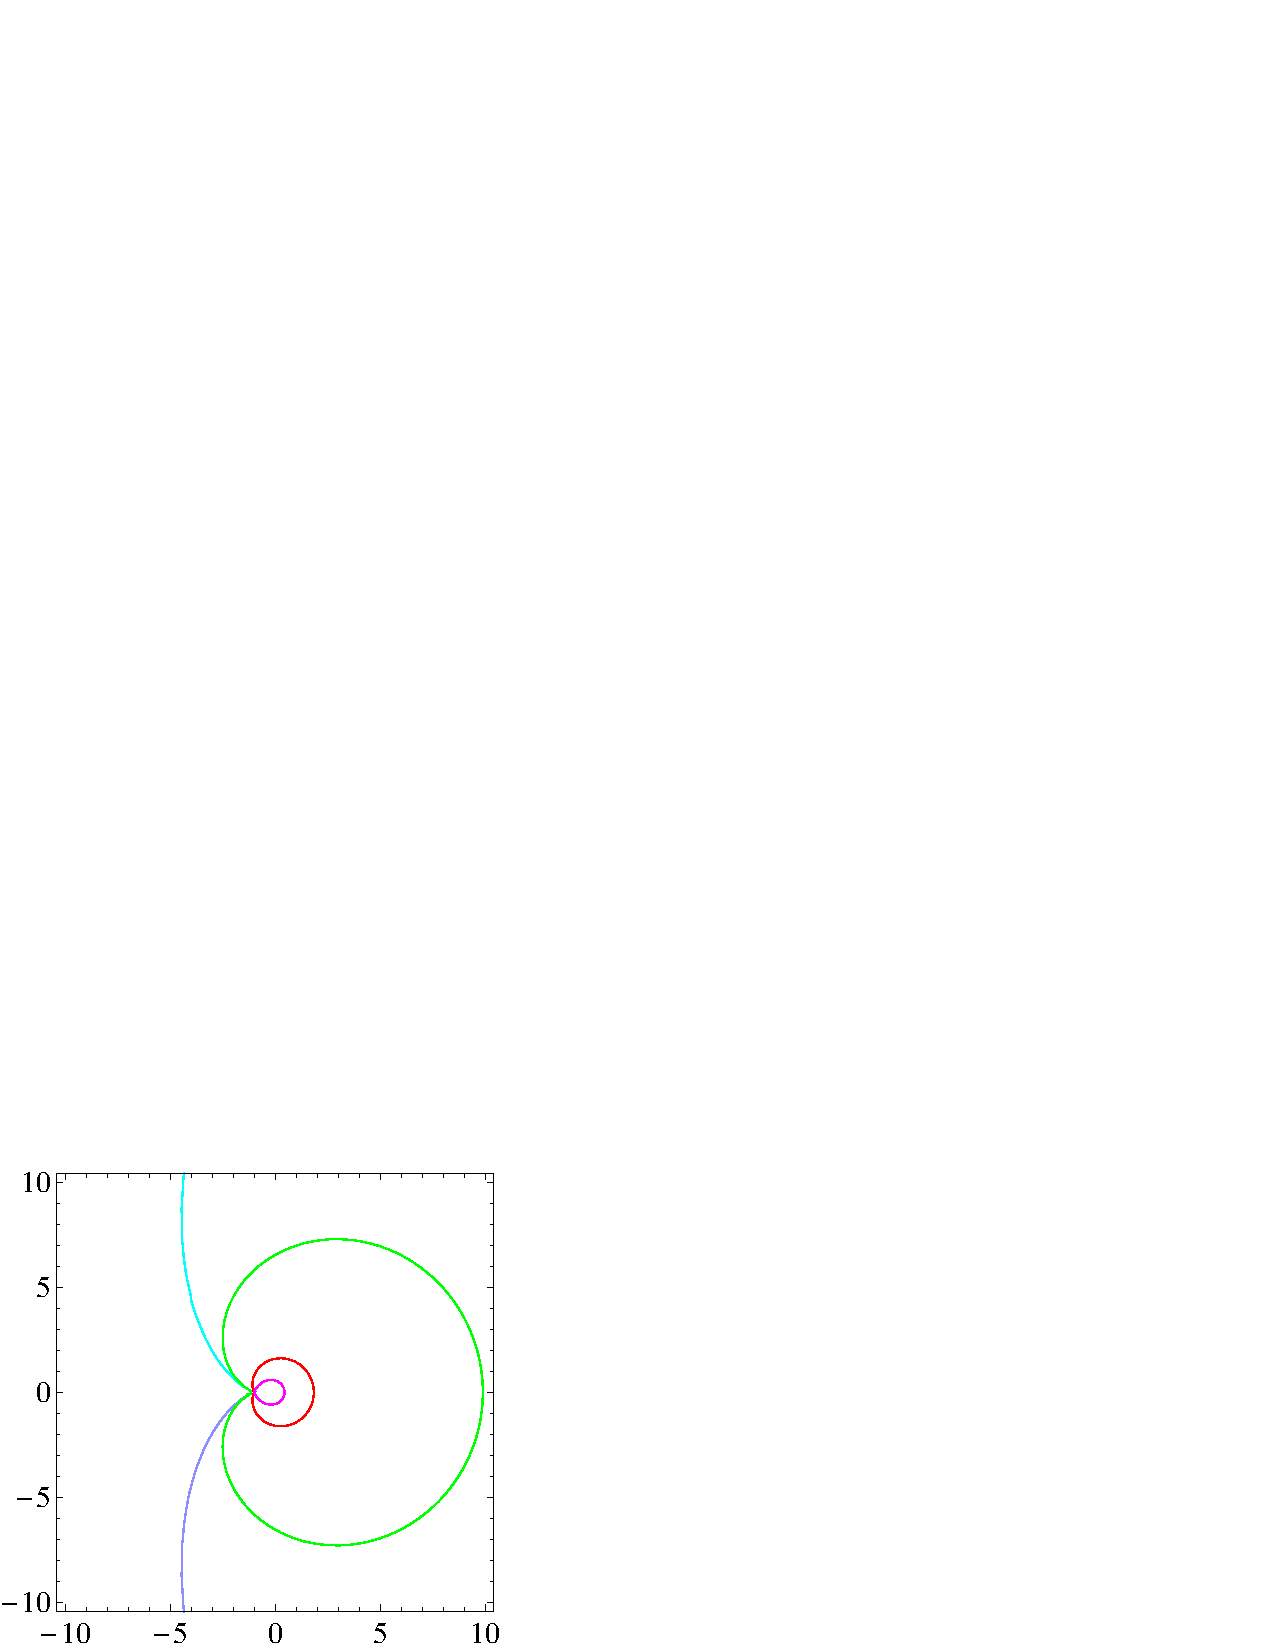
\includegraphics[width=18cm]{fdecays.pdf}
\end{center}

\end{columns}


\end{frame}


%%%%%%%%%%%%%%%%%%%%%%%%%%%%%%%%%%%%%%%%%%%%%%%%%%%%%%%%%%%%%%%%%%
\begin{frame}{Decays}

\vspace{-1.5mm}
\begin{block}{Simple decays:}
\begin{align*}
%
	~~~~~~~~~~~~~~
	\D^{(n)}\,\Q  & ~~\longrightarrow~~  \D^{(n)}  ~~~~+~~~  \Q
	\qquad\qquad~~ n ~<~ 1 
	\\[3mm]
%
	~~~~~~~~~~~~~~
	\D^{(n)}\,\Q  & ~~\longrightarrow~~  \D^{(n-1)}  ~~+~~  \wt{\Q}
	\qquad\qquad~~ n ~>~ 1 
\end{align*}
\end{block}

	\pause
\begin{block}{Topological decays:}
\begin{align*}
%
	\D_{10}^{(1)}\,\Q  & ~~\longrightarrow~~  \ov{\M}{}_{02}  ~~~+~~~  \ov{\D}{}_{21}^{(1)}
	~~~~~~
	\\[3mm]
%
	\V_{10}^2~\,        & ~~\longrightarrow~~  ~\ov{\D}{}_{02}  ~~~+~~~  \ov{\M}{}_{21}
	~~~~~~
\end{align*}
\end{block}

\end{frame}


%%%%%%%%%%%%%%%%%%%%%%%%%%%%%%%%%%%%%%%%%%%%%%%%%%%%%%%%%%%%%%%%%%
%%%%%%%%%%%%%%%%%%%%%%%%%%%%%%%%%%%%%%%%%%%%%%%%%%%%%%%%%%%%%%%%%%
\section{..Concluding}
%%%%%%%%%%%%%%%%%%%%%%%%%%%%%%%%%%%%%%%%%%%%%%%%%%%%%%%%%%%%%%%%%%
%%%%%%%%%%%%%%%%%%%%%%%%%%%%%%%%%%%%%%%%%%%%%%%%%%%%%%%%%%%%%%%%%%


%%%%%%%%%%%%%%%%%%%%%%%%%%%%%%%%%%%%%%%%%%%%%%%%%%%%%%%%%%%%%%%%%%
\begin{frame}{Generalizing to higher $ N $}

\begin{block}{}

	\vspace{2mm}
	Two states become part of the ``monopole'' tower
	\vspace{2mm}

\end{block}

\vspace{7mm}

\pause
\begin{block}{}

	\vspace{2mm}
	All extra states decay

	\vspace{1mm}
\uncover<3->{
	(Indeed for even $ N $ there are {\it no bound states})
	}	
	\vspace{2mm}

\end{block}

\vspace{7mm}

\uncover<4->{
\begin{block}{}

	\vspace{2mm}
	We can infer that most likely they decay for \underline{{\it all} $N$}
	\vspace{2mm}

\end{block}
}

\end{frame}



%%%%%%%%%%%%%%%%%%%%%%%%%%%%%%%%%%%%%%%%%%%%%%%%%%%%%%%%%%%%%%%%%%
%%%%%%%%%%%%%%%%%%%%%%%%%%%%%%%%%%%%%%%%%%%%%%%%%%%%%%%%%%%%%%%%%%
\section{.....Concluding}
%%%%%%%%%%%%%%%%%%%%%%%%%%%%%%%%%%%%%%%%%%%%%%%%%%%%%%%%%%%%%%%%%%
%%%%%%%%%%%%%%%%%%%%%%%%%%%%%%%%%%%%%%%%%%%%%%%%%%%%%%%%%%%%%%%%%%


%%%%%%%%%%%%%%%%%%%%%%%%%%%%%%%%%%%%%%%%%%%%%%%%%%%%%%%%%%%%%%%%%%
\begin{frame}{SQCD in four dimensions}

\begin{block}{}

	\vspace{2mm}
	there are also $ N $ states at strong coupling
	\vspace{2mm}

\end{block}

\vspace{7mm}

\pause
\begin{block}{}

	\vspace{2mm}
	our results indicate that two of them are part of one tower of dyons
	\vspace{2mm}

\end{block}

\vspace{7mm}

\pause
\begin{block}{}

	\vspace{2mm}
	other states decay before reaching the weak coupling
	\vspace{2mm}

\end{block}

\end{frame}


%%%%%%%%%%%%%%%%%%%%%%%%%%%%%%%%%%%%%%%%%%%%%%%%%%%%%%%%%%%%%%%%%%
%%%%%%%%%%%%%%%%%%%%%%%%%%%%%%%%%%%%%%%%%%%%%%%%%%%%%%%%%%%%%%%%%%
\section{.........Concluded}
%%%%%%%%%%%%%%%%%%%%%%%%%%%%%%%%%%%%%%%%%%%%%%%%%%%%%%%%%%%%%%%%%%
%%%%%%%%%%%%%%%%%%%%%%%%%%%%%%%%%%%%%%%%%%%%%%%%%%%%%%%%%%%%%%%%%%


%%%%%%%%%%%%%%%%%%%%%%%%%%%%%%%%%%%%%%%%%%%%%%%%%%%%%%%%%%%%%%%%%%
\begin{frame}{}

\usefont{T1}{ptm}{m}{n}\fontsize{60pt}{60pt}\selectfont
\begin{center}
        Thank you
\end{center}


\end{frame}



\end{document}
